La première expérience avec la fonction structurante cible \textit{cross3} pour l'opération cible d'ouverture et avec la banque d'images d'entraînement MNIST, expérience pour laquelle le réseau ne converge originellement pas avec une initialisation aléatoire des poids des noyaux $w$ issue d'une loi normale centrée réduite, s'avère ici être un succès grâce à l'initialisation gaussienne 2D de ces noyaux (voir figure précédente \ref{fig:init_gauss}). 
Cependant, pour estimer avec davantage de certitude l'efficacité globale de cette modulation de l'initialisation des noyaux $w$ des couches du réseau, il faut observer son impact sur l'ensemble des expériences de notre étude, donc également sur les expériences qui sont originellement un succès avec une initialisation aléatoire des $w$. \\

\vspace{-1.0mm}
\noindent Considérons alors ici le même paramétrage du réseau $\mathcal{S}$MorphNetTanh à deux couches morphologiques que dans la partie précédente, c'est-à-dire munie, dans la fonction de perte \textit{loss}, d'un partage de poids doux entre les noyaux $w$ de ses deux couches (formule \ref{Csim3}), et de la contrainte $C_\text{awayOPP}$ sur l'éloignement opposé entre ses deux paramètres de contrôle $\alpha$ respectifs (formule \ref{erreur_awayOPP}). On modifie donc simplement ici, sur l'ensemble des expériences de notre étude, l'initialisation des poids des noyaux $w$ par une gaussienne 2D telle que décrite précédemment (illustrée fig. \ref{fig:init_gauss} en début d'entraînement, sur la seconde ligne, à 0\%), et les résultats de convergence issus de cette initialisation déterministe sont comparés à ceux issus de l'initialisation aléatoire. \\

\vspace{-1.0mm}
En reprenant donc la même méthodologie que précédemment avec des réseaux $\mathcal{S}$MorphNetTanh à deux couches, on obtient, pour l’opération cible d’ouverture et la banque d’images d’entraînement MNIST, les résultats suivants (fig. \ref{fig:RANDvsGAUSS_opening}) : \\


% figure
\vspace{0.1mm}
\begin{figure}[!htp]
  \begin{center}
    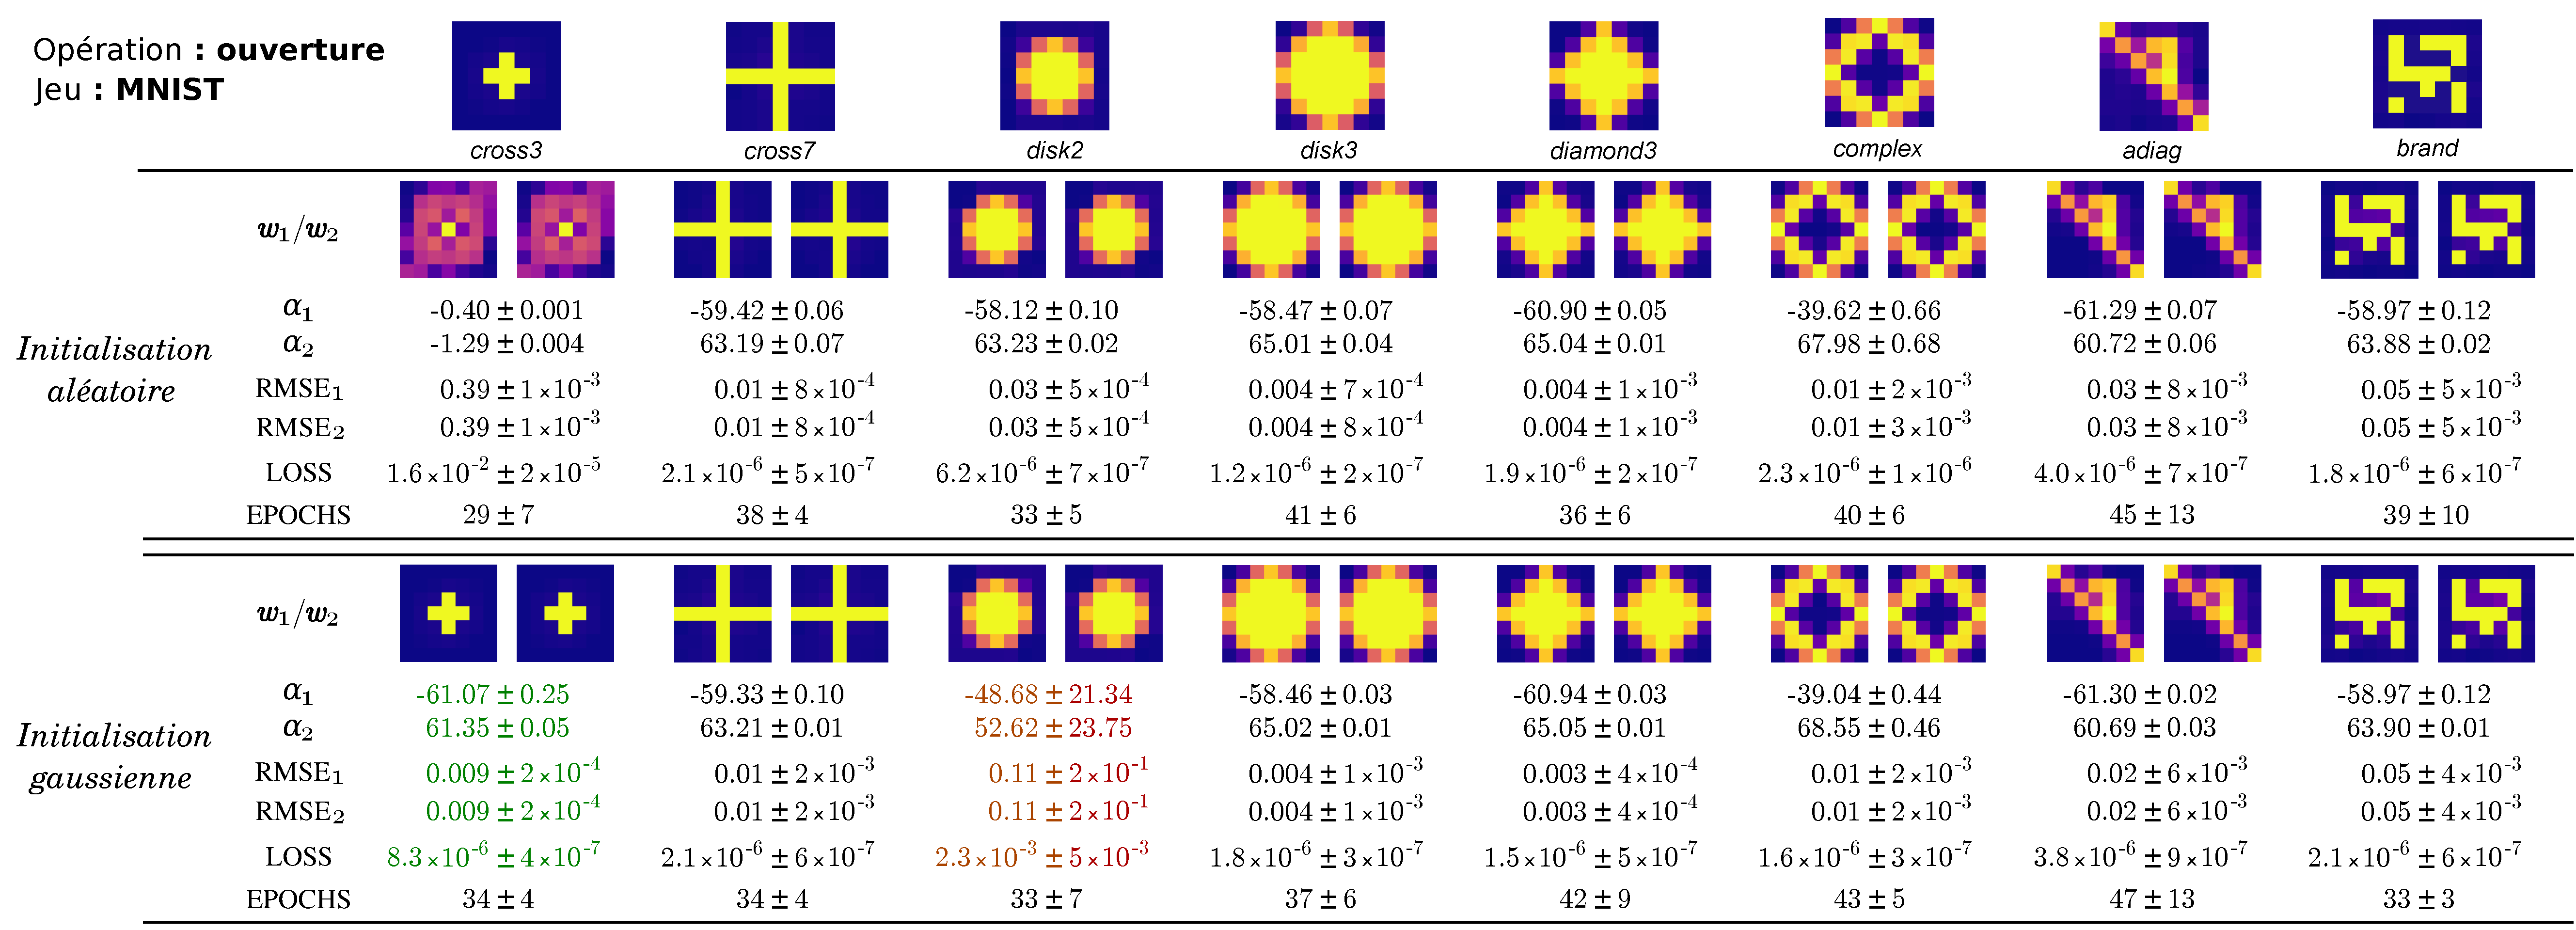
\includegraphics[width=1.00\linewidth]{parts/3-contributions/D-modulation_de_l_initialisation/figures/g_opening_mnist.pdf}
    \vspace{-4.0mm}
    \caption{ \centering Comparaison des poids appris et des moyennes et écarts-types des métriques $\alpha$, \textit{RMSE}, \textit{loss} et nombre d'époques, et ce sur six runs, entre initialisation aléatoire et gaussienne, pour les huit fonctions structurantes cibles et l'opération d'\textbf{ouverture}.}
    \label{fig:RANDvsGAUSS_opening}
  \end{center}
\end{figure}


\newpage

On obtient également, pour l’opération cible de fermeture et la banque MNIST avec des réseaux $\mathcal{S}$MorphNetTanh à deux couches, les résultats suivants (fig. \ref{fig:RANDvsGAUSS_closing}) : \\

%figure
\vspace{0.2mm}
\begin{figure}[!htp]
  \begin{center}
    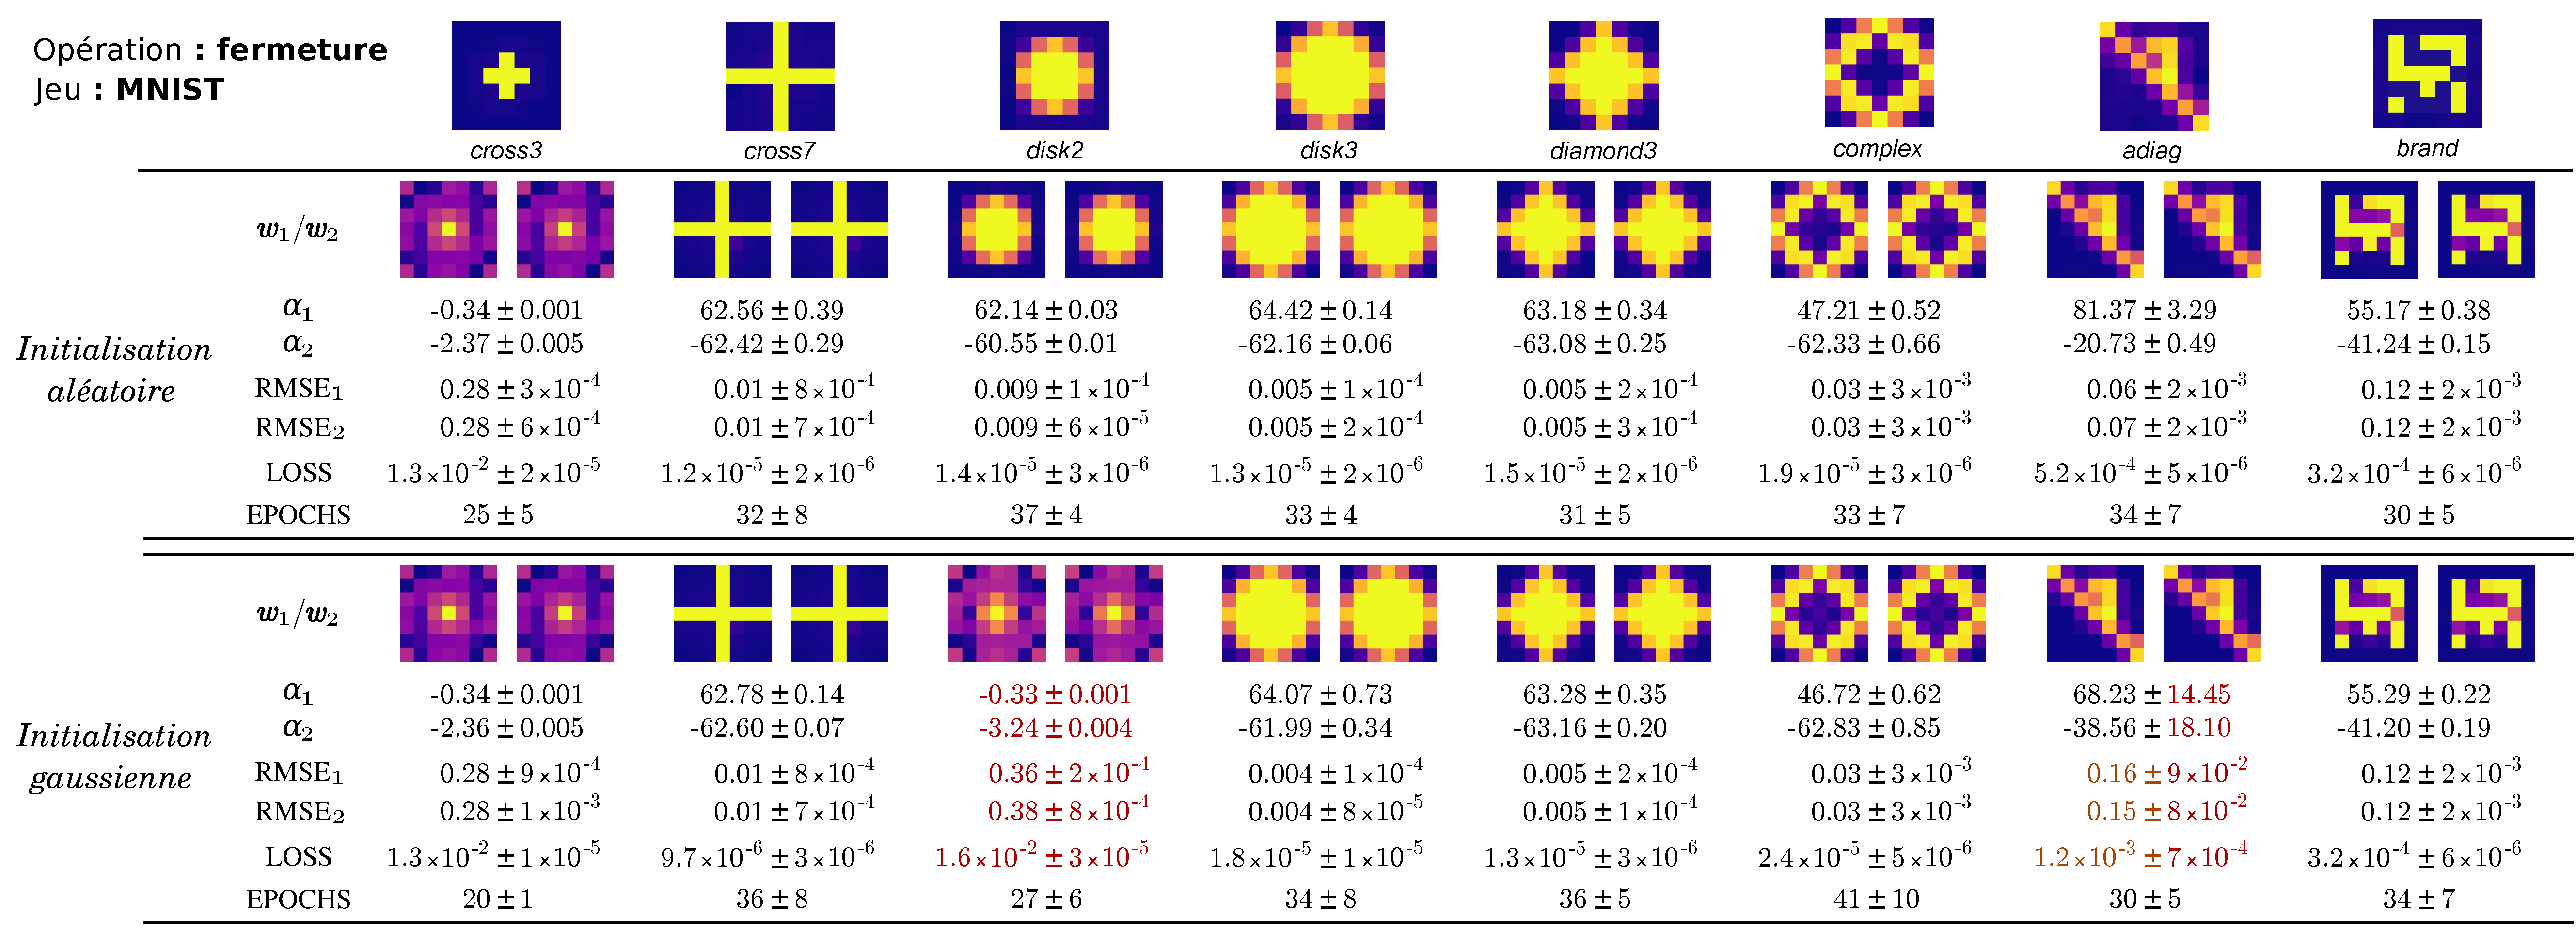
\includegraphics[width=1.00\linewidth]{parts/3-contributions/D-modulation_de_l_initialisation/figures/g_closing_mnist.pdf}
    \vspace{-4.0mm}
    \caption{ \centering Comparaison des poids appris et des moyennes et écarts-types des métriques $\alpha$, \textit{RMSE}, \textit{loss} et nombre d'époques, et ce sur six runs, entre initialisation aléatoire et gaussienne, pour les huit fonctions structurantes cibles et l'opération de \textbf{fermeture}.}
    \label{fig:RANDvsGAUSS_closing}
  \end{center}
\end{figure}


\vspace{-2.0mm}
Les données en rouge illustrent les cas où l'initialisation gaussienne donne de moins bons résultats que l'initialisation aléatoire, tandis que ceux en vert illustrent, à inverses, les cas où c'est l'initialisation gaussienne qui donne de meilleurs résultats. \\ %que l'aléatoire.

\vspace{-2.2mm}
\noindent On remarque en effet que l'expérience avec \textit{cross3} pour l'ouverture avec MNIST est un net succès pour l'initialisation gaussienne contrairement à l'initialisation aléatoire, aussi bien en terme visuel avec une grande ressemblance des noyaux $w$ par rapport à la structure cible \textit{cross3}, qu'en termes de valeurs des métriques de performances, avec une \textit{RMSE} bien plus faible pour les deux noyaux $w$, une forte valeur absolue des deux paramètres de contrôle $\alpha$ avec le bon signe, et une perte globale \textit{loss} mineure. \\

\vspace{-2.2mm}
\noindent Cependant, il s'agit là de la seule expérience dont les résultats sont meilleurs avec l'initialisation gaussienne. Il y a, à l'inverse, plusieurs expériences qui ont cette fois moins bien convergé avec une telle initialisation, telles que celles avec \textit{disk2} à la fois pour l'ouverture et la fermeture, ou encore celle avec \textit{adiag} pour la fermeture (qui a des écarts-types élevés, illustrant l'échec de certaines runs), sur MNIST. Certains succès avec une initialisation aléatoire sont ainsi devenus des échecs avec la gaussienne. \\

\vspace{-1.6mm}
En conclusion, on ne peut pas dire que l'initialisation aléatoire donne de meilleurs résultats de convergence sur ces réseaux, d'autant plus que l'on obtient les mêmes résultats, voir pires, avec la banque FashionMNIST. On s'interroge en particulier sur la raison de l'échec des expériences avec la structure cible \textit{disk2}, qui a pourtant une forme visuelle proche de la gaussienne 2D utilisée pour l'initialisation des noyaux $w$.
